% ==== Document Class & Packages =====
\documentclass[12pt,hidelinks]{article}
	\usepackage[explicit]{titlesec}
	\usepackage{titletoc}
	\usepackage{tocloft}
	\usepackage{charter}
	\usepackage[many]{tcolorbox}
	\usepackage{amsmath}
	\usepackage{graphicx}
	\usepackage{xcolor}
	\usepackage{tikz,lipsum,lmodern}
	\usetikzlibrary{calc}
	\usepackage[hungarian]{babel}
	\usepackage{fancyhdr}
	\usepackage{mathrsfs}
	\usepackage{empheq}
	\usepackage{fourier}% change to lmodern if fourier is no available
	\usepackage{wrapfig}
	\usepackage{fancyref}
	\usepackage{hyperref}
	\usepackage{cleveref}
	\usepackage{listings}
	\usepackage{varwidth}
	\usepackage{longfbox}
	\usepackage{geometry}
	\usepackage{marginnote}
	\tcbuselibrary{theorems}
	\tcbuselibrary{breakable, skins}
	\tcbuselibrary{listings, documentation}
	\geometry{
		a4paper,
		left=33mm,
		right=33mm,
		top=20mm}
% ========= Path to images ============
%   - Direct the computer on the path 
% 	  to the folder containg the images
% =====================================
\graphicspath{{./images/}}
% ============= Macros ================
\newcommand{\fillin}{\underline{\hspace{.75in}}{\;}}
\newcommand{\solution}{\textcolor{mordantred19}{Solution:}}
\setlength{\parindent}{0pt}
\addto{\captionsenglish}{\renewcommand*{\contentsname}{Table of Contents}}
\linespread{1.2}
% ======== Footers & Headers ==========
\cfoot{\thepage}
\chead{}\rhead{}\lhead{}
% =====================================
\renewcommand{\thesection}{\arabic{section}}
\newcommand\sectionnumfont{% font specification for the number
	\fontsize{90}{40}\color{section_low}\selectfont}
\newcommand\sectionnamefont{% font specification for the name "PART"
	\normalfont\color{white}\scshape\small\bfseries }
% ============= Colors ================
% ----- Red -----
\definecolor{mordantred19}{rgb}{0.68, 0.05, 0.0}
% ----- Blue -----
\definecolor{st.patrick\'sblue}{rgb}{0.14, 0.16, 0.48}
\definecolor{teal}{rgb}{0.0, 0.5, 0.5}
\definecolor{beaublue}{rgb}{0.74, 0.83, 0.9}
\definecolor{aut_red}{RGB}{192,0,0}
\definecolor{myblueii}{RGB}{63,0,244}
\definecolor{section_low}{RGB}{220,220,220}
% ---- Yellow ----
\definecolor{blond}{rgb}{0.98, 0.94, 0.75}
\definecolor{cream}{rgb}{1.0, 0.99, 0.82}
% ----- Green ------
\definecolor{emerald}{rgb}{0.31, 0.78, 0.47}
\definecolor{darkspringgreen}{rgb}{0.09, 0.45, 0.27}
% ---- White -----
\definecolor{ghostwhite}{rgb}{0.97, 0.97, 1.0}
\definecolor{splashedwhite}{rgb}{1.0, 0.99, 1.0}
% ---- Grey -----
\definecolor{whitesmoke}{rgb}{0.96, 0.96, 0.96}
\definecolor{lightgray}{rgb}{0.92, 0.92, 0.92}
\definecolor{floralwhite}{rgb}{1.0, 0.98, 0.94}
% ========= Part Format ==========
\titleformat{\section}
{\normalfont\huge\filleft}
{}
{20pt}
{\begin{tikzpicture}[remember picture,overlay]
	\fill[section_low] 
	(current page.north west) rectangle ([yshift=-5.5cm]current page.north east);   
\node[
	fill=aut_red,
	text width=2\paperwidth,
	rounded corners=2cm,
	text depth=5cm,
	anchor=center,
	inner sep=0pt] at (current page.north east) (parttop)
	{\thepart};%
\node[
	anchor=south east,
	inner sep=0pt,
	outer sep=0pt] (partnum) at ([xshift=-20pt]parttop.south) 
	{\sectionnumfont\thesection};
\node[
	anchor=north east,
	align=right,
	inner xsep=0pt] at ([yshift=-0.5cm]partname.east|-partnum.south) 
	{\parbox{.7\textwidth}{\raggedleft#1}};
\end{tikzpicture}%
}
% ========= Hyper Ref ===========
\hypersetup{
	colorlinks,
	linkcolor={red!50!black},
	citecolor={blue!50!black},
	urlcolor={blue!80!black}
}
% ========= Example Boxes =============
\tcbset{
	defstyle/.style={
		fonttitle=\bfseries\upshape, 
		fontupper=\slshape,
		arc=0mm, 
		beamer,
		colback=blue!5!white,
		colframe=blue!75!black},
	theostyle/.style={
		fonttitle=\bfseries\upshape, 
		fontupper=\slshape,
		colback=red!10!white,
		colframe=red!75!black},
	visualstyle/.style={
		height=6.5cm,
		breakable,
		enhanced,
		leftrule=0pt,
		rightrule=0pt,
		bottomrule=0pt,
		outer arc=0pt,
		arc=0pt,
		colframe=mordantred19,
		colback=lightgray,
		attach boxed title to top left,
		boxed title style={
			colback=mordantred19,
			outer arc=0pt,
			arc=0pt,
			top=3pt,
			bottom=3pt,
		},
		fonttitle=\sffamily,},
	discussionstyle/.style={
		height=6.5cm,
		breakable,
		enhanced,
		rightrule=0pt,
		toprule=0pt,
		outer arc=0pt,
		arc=0pt,
		colframe=mordantred19,
		colback=lightgray,
		attach boxed title to top left,
		boxed title style={
			colback=mordantred19,
			outer arc=0pt,
			arc=0pt,
			top=3pt,
			bottom=3pt,
		},
		fonttitle=\sffamily},
	mystyle/.style={
		height=6.5cm,
		breakable,
		enhanced,
		rightrule=0pt,
		leftrule=0pt,
		bottomrule=0pt,
		outer arc=0pt,
		arc=0pt,
		colframe=mordantred19,
		colback=lightgray,
		attach boxed title to top left,
		boxed title style={
			colback=mordantred19,
			outer arc=0pt,
			arc=0pt,
			top=3pt,
			bottom=3pt,
		},
		fonttitle=\sffamily},
	aastyle/.style={
			height=3.5cm,
			enhanced,
			colframe=teal,
			colback=lightgray,
			colbacktitle=floralwhite,
			fonttitle=\bfseries,
			coltitle=black,
		attach boxed title to top center={
	  		yshift=-0.25mm-\tcboxedtitleheight/2,
	   		yshifttext=2mm-\tcboxedtitleheight/2}, 
		boxed title style={boxrule=0.5mm,
			frame code={ \path[tcb fill frame] ([xshift=-4mm]frame.west)
				-- (frame.north west) -- (frame.north east) -- ([xshift=4mm]frame.east)
				-- (frame.south east) -- (frame.south west) -- cycle; },
			interior code={ 
				\path[tcb fill interior] ([xshift=-2mm]interior.west)
				-- (interior.north west) -- (interior.north east)
				-- ([xshift=2mm]interior.east) -- (interior.south east) -- (interior.south west)
				-- cycle;} }
				},
	examstyle/.style={
		height=9.5cm,
		breakable,
		enhanced,
		rightrule=0pt,
		leftrule=0pt,
		bottomrule=0pt,
		outer arc=0pt,
		arc=0pt,
		colframe=mordantred19,
		colback=lightgray,
		attach boxed title to top left,
		boxed title style={
			colback=mordantred19,
			outer arc=0pt,
			arc=0pt,
			top=3pt,
			bottom=3pt,
		},
		fonttitle=\sffamily},
	doc head command={
		interior style={
			fill,
			left color=yellow!20!white, 
			right color=white}},
	doc head environment={
		boxsep=4pt,
		arc=2pt,
		colback=yellow!30!white,
		},
	doclang/environment content=text
}
% ============= Boxes ================
\newtcolorbox[auto counter,number within=section]{example}[1][]{
	mystyle,
	title=Example~\thetcbcounter,
	overlay unbroken and first={
		\path
		let
		\p1=(title.north east),
		\p2=(frame.north east)
		in
		node[anchor=
			west,
			font=\sffamily,
			color=st.patrick\'sblue,
			text width=\x2-\x1] 
		at (title.east) {#1};
	}
}
\newtcolorbox[auto counter,number within=section]{longexample}[1][]{
	examstyle,
	title=Example~\thetcbcounter,
	overlay unbroken and first={
		\path
		let
		\p1=(title.north east),
		\p2=(frame.north east)
		in
		node[anchor=
		west,
		font=\sffamily,
		color=st.patrick\'sblue,
		text width=\x2-\x1] 
		at (title.east) {#1};
	}
}
\newtcolorbox[auto counter,number within=section]{example2}[1][]{
	aastyle,
	title=Example~\thetcbcounter,{}
}
\newtcolorbox[auto counter,number within=section]{discussion}[1][]{
	discussionstyle,
	title=Discussion~\thetcbcounter,
	overlay unbroken and first={
		\path
		let
		\p1=(title.north east),
		\p2=(frame.north east)
		in
		node[anchor=
		west,
		font=\sffamily,
		color=st.patrick\'sblue,
		text width=\x2-\x1] 
		at (title.east) {#1};
	}
}
\newtcolorbox[auto counter,number within=section]{visualization}[1][]{
	visualstyle,
	title=Visualization~\thetcbcounter,
	overlay unbroken and first={
		\path
		let
		\p1=(title.north east),
		\p2=(frame.north east)
		in
		node[anchor=
		west,
		font=\sffamily,
		color=st.patrick\'sblue,
		text width=\x2-\x1] 
		at (title.east) {#1};
	}
}
% --------- Theorems ---------
\newtcbtheorem[number within=subsection,crefname={definition}{definitions}]%
	{Definition}{Definition}{defstyle}{def}%
\newtcbtheorem[use counter from=Definition,crefname={theorem}{theorems}]%
	{Theorem}{Theorem}{theostyle}{theo}
	%
\newtcbtheorem[use counter from=Definition]{theo}{Theorem}%
{
	theorem style=plain,
	enhanced,
	colframe=blue!50!black,
	colback=yellow!20!white,
	coltitle=red!50!black,
	fonttitle=\upshape\bfseries,
	fontupper=\itshape,
	drop fuzzy shadow=blue!50!black!50!white,
	boxrule=0.4pt}{theo}
\newtcbtheorem[use counter from=Definition]{DashedDefinition}{Definition}%
 {
 	enhanced,
 	frame empty,
 	interior empty,
 	colframe=darkspringgreen!50!white,
	coltitle=darkspringgreen!50!black,
	fonttitle=\bfseries,
	colbacktitle=darkspringgreen!15!white,
	borderline={0.5mm}{0mm}{darkspringgreen!15!white},
	borderline={0.5mm}{0mm}{darkspringgreen!50!white,dashed},
	attach boxed title to top center={yshift=-2mm},
	boxed title style={boxrule=0.4pt},
	varwidth boxed title}{theo}
%%%%%%%%%%%%%%%%%%%%%%%%%%%%%%%%%%%%%%%%
\newtcblisting[auto counter,number within=section]{disexam}{
	skin=bicolor,
	colback=white!30!beaublue,
	colbacklower=white,
	colframe=black,
	before skip=\medskipamount,
	after skip=\medskipamount,
	fontlower=\footnotesize,
	listing options={style=tcblatex,texcsstyle=*\color{red!70!black}},}
%%%%%%%%%%%%%%%%%%%%%%%%%%%%%%%%%%%%%%%


\begin{document}
\begin{titlepage}
	\centering % Center everything on the title page
	\scshape % Use small caps for all text on the title page
	\vspace*{1.5\baselineskip} % White space at the top of the page
% ===================
%	Title Section 	
% ===================

	\rule{13cm}{1.6pt}\vspace*{-\baselineskip}\vspace*{2pt} % Thick horizontal rule
	\rule{13cm}{0.4pt} % Thin horizontal rule
	
		\vspace{0.75\baselineskip} % Whitespace above the title
% ========== Title ===============	
	{	\Huge Irányítástechnika Eszközei\\	}
% ======================================
		\vspace{0.75\baselineskip} % Whitespace below the title
	\rule{13cm}{0.4pt}\vspace*{-\baselineskip}\vspace{3.2pt} % Thin horizontal rule
	\rule{13cm}{1.6pt} % Thick horizontal rule
	
		\vspace{1.75\baselineskip} % Whitespace after the title block
% =================
%	Information	
% =================
	{\large David Kiss \\
		\vspace*{1.2\baselineskip}
	david.kiss@aut.bme.hu} \\
	\vfill

\end{titlepage}
%%%%%%%%%%%%%%%%%%%%%%%%%%%%%%%%%%%%%%%%%%%%%%%%%%%%%%%%%%%
\tableofcontents
\vfill
\small{\noindent \textbf{A jegyzetről} \vspace{-3mm}\\
\noindent \rule{3.3cm}{0.5pt} \\
A dokuemtum folyamatos fejlődés alatt áll}
\newpage

\section{Bevezető}
\vspace{4cm}

\vspace{-1.5mm}
\newpage
\section{Analóg elektronikai alapismeretek}
\vspace{4cm}

\vspace{-1.5mm}
\newpage
\section{Digitális technika alpajai}
\vspace{5cm}

Az előző fejezetben megismert analóg elektronikai ismeretek segítségével sok irányítási és szabályozási probléma megoldható, azonban ezek használata ma már csak szék és speciális körökre korlátozódik, az analóg szabályzások helyét a digitális megoldások vették át. Ennek ok, hogy a digitális iránytó rendszerek jellemzően sokkal nagyobb flexibilitást kínálnak, hiszen az adott rendszer később is tetszőlegesen újraporgramozható. A beágyazott mikorvezérlők terjedésével pedig a költségük is rendkívül alacsony, illetve nem szabad megfeletkezni arról sem, hogy az ilyen, digitális irányító egységgel ellátott rendszerek komplexitása jellemzően sokkal alacsonyabb, hiszen a több 10-100 alaktrészből álló analóg szabályzót egy darab CPU helyettesíti, amely elvégiz a szükséges számításokat. A digitális és az analóg világ közti átmenet azonban kihívsáokat rejt magában. Míg az analóg jelek információtartalmát gyakorlatilag a zajterheltség és a sávszélesség határozza meg, addig digitális esetben számolnunk kell az ábrázolás \emph{bitmélységével}, ileltve a \emph{mintavételi idővel}. A digitális jelekre való konverzió nem veszteségmentes, az eredeti jel teljes valójába nem állíthaó vissza.

\subsection{Digitális jelek}

\subsection{Digitális számábrázolás}
\subsubsection{Számrendszerek}
\subsubsection{Negatív számok ábárzolása}
\subsubsection{Tört számok ábárázolása}
\subsubsection{Egyéb numerikus kódolások}
\paragraph{BCD kódolás}
\paragraph{Gray-kód}
\subsection{Digitális logika}
\subsection{Kombinációs logikai hálózatok}

\begin{example2}[\quad \large Logikai kapuk]

Soroljon fel 6 fajta logikai kaput! Valósítson meg egy 2 bites összeadót! Átvitellel nem kell számolni.


\end{example2}

AND, OR, NAND, NOR, NOT, XOR, ezek rajzjelei, igazságtáblája és logikai jelölése.

\subsubsection{Alapvető logikai kapuk}
\subsubsection{Logikai függvények leírása}
\subsubsection{Logikai függvények egyszerűsítése}
\subsection{Sorrendi logikai hálózatok}

\begin{example}[\quad \large 2 bites összeadó]

Valósítsa meg az alábbi 1kimenetű 2 bemenetű funkciót NAND kapuk felhasználásával: Q=1, ha S=1, Q=0, ha S=0 és nR=0, egyébként Q megőrzi addigi értékét!

\tcbline
\vspace{1mm}

\solution

\end{example}
\begin{example}[\quad \large Sorrendi logikai hálózatok 2.]

Valósítsa meg az alábbi 1kimenetű 3 bemenetű funkciót logikai kapuk és D tárolók felhasználásával: a CLK bemenet felfutó élét követően Q=1, ha S=1, Q=0, ha S=0 és R=1, egyébként Q megőrzi addigi értékét!

\tcbline
\vspace{1mm}

\solution

\end{example}
\begin{example}[\quad \large 2 bites összeadó]

D tároló(k) és NAND kapu(k) felhasználásával valósítsa meg a következő funkciót:
A CLK órajel felfutó élénél a Q kimenet megváltoztatja értékét, ha az EN bemenet 1, ellenkező esetben Q állapota változatlan marad.


\tcbline
\vspace{1mm}

\solution

\end{example}
\begin{example}[\quad \large Sorrendi logikai hálózatok 3.]

D tároló(k) és NAND kapu(k) felhasználásával valósítsa meg a következő funkciót:
A CLK órajel felfutó élénél a két Q kimenet rendre az alábbi értékeket veszi fel: 00, 01, 10, 11, 00…


\tcbline
\vspace{1mm}

\solution

\end{example}
\begin{example}[\quad \large 2 bites összeadó]

Készítsen 2 bites számlálót D tárolók és NAND kapuk felhasználásával! 

\tcbline
\vspace{1mm}

\solution

\end{example}




\vspace{-1.5mm}
\newpage
\section{Elektronikus érzékelők}
\vspace{5cm}
\subsection{Feszültségmérésre visszavezethető mérési eljárások}

\begin{example2}[\quad \large Közvetelen érzékelők 1.]

Egy kapcsolóüzemű tápegység szűretlen kimenő feszültségét nagy pontossággal és jó dinamikával szeretnénk mérni. A kimenet és a vezérlő elektronika tápja egy ponton összeköthető. Javasoljon érzékelési módszert és méretezze az érzékelőt! ($Ui=0..100V, Uo=0..5V$, előírt pontosság 1\%, az A/D váltó bemeneti árama 1uA(max), bemeneti kapacitása 50pF(max.).
\end{example2}
Első lépésben gyűjtsük ki a szükséges paramétereket, a jelölések értelmezéséhez a \ref{fig:volt_div_sol}. ábra szolgál segítségül:
\begin{equation}
\begin{aligned}{}
    U_{in} &= 0..100\; V; \\
    U_o &= 0..5\; V; \\
    C_{AD} &= 50\; pF; \\
    I_{AD} &= 1\; \mu{}A; \\
    \alpha{} &= 1\; \%; \\
\end{aligned}
\end{equation}

Ezek után meghatározzuk a feszültésgosztáshoz székséges ellenállások mértékét a feszültésgosztó képlettel.

\begin{equation}
\begin{aligned}{}
    U_{o} &= U_{in} \cdot \frac{R_2}{R_1 + R_2} \\
\end{aligned}
\end{equation}

Mivel ebben az egyenletben két ismeretlen van, így a megoldáshoz $R_1$ és $R_2$ értéke közül az egyiket nekünk kell megválasztanunk. A gyakorlatban ezeket az ártákeket általában úgy választjuk meg, hogy a feszültésgosztó árama kelleően kicsi legyen, elkerülve a nagy teljesítmény disszipációt, viszont ne túl kicsi ahhoz, hogy túlságosan zavarérzékeny legyen. Ebben a feladatban meg van adva az elvárt pontásság $\alpha{} = 1 \%$, illetve az AD váltó által felvett áram maximális értéke $I_{AD} = 1 \mu{}A$. Ezt értelmezhetjük úgy, hogy az AD váltó áramfelvétele, maxmim $1\%$ mértékben változtathatja meg a feszültségosztó áramát, tehát $R_2$ áramának legalább a 100 szorosának kell lennie $I_{AD}$-nak.

\begin{equation}
\begin{aligned}{}
    I_{R2} &\geq I_{AD} \cdot \alpha{} \\
    \frac{U_o}{I_{R2}} &\geq \frac{U_o}{I_{AD}} \cdot \alpha{} \\
    R_{2} &\geq \frac{U_o}{I_{AD}} \cdot \alpha{} = \frac{5\;V}{1\;\mu{}A} \cdot \frac{1}{100} = 50\; k\Omega{} \\
    R_2 &= \underline{\underline{50\; k\Omega{}}}
\end{aligned}
\end{equation}

$R_2$ ismeretében már a feladat egyértelmúen megoldható:

\begin{equation}
\begin{aligned}{}
    U_{o} &= U_{in} \cdot \frac{R_2}{R_1 + R_2} \\
    R_{1} &= \frac{U_i \cdot R_2 - U_1 \cdot R_2}{U_o} = \frac{100\;V \cdot 50\; k\Omega{} - 5\; V \cdot 50\; k\Omega{}}{5 \;V} = \underline{\underline{950 \; k\Omega{}}} \\
\end{aligned}
\end{equation}

Innen már nincs más hátra, mint elvégezni a frekvenciakompenzációt.

\begin{equation}
\begin{aligned}{}
    R_1 \cdot C_1 &=  R_2 \cdot C_2 \\
    C_2 &= C_{AD} \\
    C_1 &= \frac{R_2 \cdot C_2}{R_1} = \frac{50\; k\Omega \cdot 50\; pF}{950;\ k\Omega} = \underline{\underline{2,63\; pF}}
\end{aligned}
\end{equation}

Ezzel pedig a feladat el is készült.

\begin{figure}[htb]
\begingroup
\tikzset{}
 \centerline{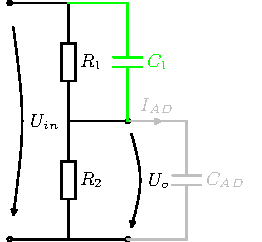
\includegraphics[width=0.4\columnwidth]{.//Figures/Tikz/tikz_voltage_divider.pdf}}
 \endgroup
 \caption{Feszültségosztó}
 \label{fig:volt_div_sol}
\end{figure}
\begin{example}[\quad \large Közvetelen érzékelők 2.]

Egy nagyfeszültségű impulzusgenerátor kimenő feszültségét nagy pontossággal és jó dinamikával szeretnénk mérni. Tervezzen galvanikusan nem leválasztott feszültség érzékelőt, ha a kimenet és a vezérlő elektronika nulla pontja azonos, $Ui=0..100V$, $Uo=0..5V$, előírt statikus pontosság 1\%, dinamikus pontosság 2\%, az A/D váltó statikus bemeneti árama $0-10uA$, bemenetére redukált kapacitás $25-50pF$!

\tcbline
\vspace{1mm}

\solution

\end{example}
\begin{example}[\quad \large Közvetelen érzékelők 3.]

Egy nagyfeszültségű impulzusgenerátor kimenő feszültségét nagy pontossággal és jó dinamikával szeretnénk mérni. Tervezzen galvanikusan nem leválasztott feszültség érzékelőt, ha a kimenet és a vezérlő elektronika nulla pontja azonos, Ui=0..1kV, $Uo=0..3V$, előírt pontosság 2\%, az A/D váltó statikus bemeneti árama 1uA(max), bemenetére redukált kapacitás 50pF(max.)!

\tcbline
\vspace{1mm}

\solution

\end{example}
\begin{example}[\quad \large Közvetelen érzékelők 4.]

Egy nagy kapcsolási frekvenciával működő DC/DC átalakító kimenő feszültségét nagy pontossággal és jó dinamikával szeretnénk mérni. A kimenet és a vezérlő elektronika tápja egy ponton összeköthető. Javasoljon érzékelési módszert és méretezze az érzékelőt! (Ui=0..100V, Uo=0..5V, előírt pontosság 1\%, az A/D váltó bemeneti árama 1uA(max), bemeneti kapacitása 50pF(max.).

\tcbline
\vspace{1mm}

\solution

\end{example}
\begin{example}[\quad \large Közvetelen érzékelők 1]

Egy nagyfeszültségű impulzusgenerátor kimenő feszültségét nagy pontossággal és jó dinamikával szeretnénk mérni. A kimenet és a vezérlő elektronika tápja egy ponton összeköthető. Javasoljon érzékelési módszert és adja meg a méretezési szempontokat!

\tcbline
\vspace{1mm}

\solution

\end{example}
\begin{example}[\quad \large Közvetelen érzékelők 6.]

Egy nagyfrekvenciás nagyfeszültségű jelet nagysebességű A/D váltóval kívánunk mintavételezni. Milyen érzékelőt használ, ha galvanikus leválasztás nem szükséges?

\tcbline
\vspace{1mm}

\solution

\end{example}
\begin{example}[\quad \large Közvetelen érzékelők 7.]

Közvetlen áramérzékelést valósítunk meg egy 10mOhm-os sönt-ellenállással. A sönt-ellenállás induktivitása 1μH. Rajzoljon fel egy olyan kapcsolást, amely a söntön átfolyó 0-10A-es tartományt az AD váltó 0-5V-os tartományába konvertálja és dinamikusan is helyes eredményt ad!

\tcbline
\vspace{1mm}

\solution

\end{example}
\begin{example}[\quad \large Közvetelen érzékelők 1]

Tervezzen 0A és +1A között változó áram érzékelésére alkalmas galvanikusan nem leválasztó érzékelőt 2 kivezetéses söntellenállás felhasználásával! A söntellenállás mérőpontjai közötti ellenállás 100mOhm, a söntellenállás induktivitása 0,1uH. A kimeneti feszültségtartomány 0..5V legyen! A műveleti erősítő milyen tulajdonságára kell odafigyelni, ha az előírt statikus pontosság 0,5\%?

\tcbline
\vspace{1mm}

\solution

\end{example}

\subsubsection{Galvanikusan csatolt mérési elrendezések}

\begin{example}[\quad \large Közvetelen érzékelők 1]

Egy 0-100Hz-es tartományban 42V DC feszültségről üzemelő frekvenciaváltó (inverter) kimeneti áramát kell érzékelnünk. Tervezzen és méretezzen olyan érzékelő áramkört, amely a maximum 1A-es kimeneti áram pillanatértéket feltételezve a szükséges mérési tartományban az árammal arányos jelet az A/D váltó 0-5V-os bemeneti tartományába konvertálja! Galvanikusan leválasztás nem szükséges. Az előírt érzékelési pontosság 100mA.

\tcbline
\vspace{1mm}

\solution

\end{example}
\begin{example2}[\quad \large Nem leválasztott érzékelők 2.]

Egy árammérő söntellenellás jellemzői: $Rs=10\;m\Omega{}$, $Ls=0.1\;\mu{}H$. Tervezzen illesztőáramkört, amely a $0..5\;A$ mérési tartományt az AD váltó bemenetére közel frekvenciafüggetlen módon $0..5\;V$-os tartományba alakítja! A sönt 4 kivezetéses, főáramköri negatív pontja közös a jelfeldolgozó elektronika nulla pontjával.

\end{example2}

A feladatban egy árammérő söntöt kell egyfelől jelillesztenünk, másfelől pedig frekvencia kompenzálnunk. Az alábbi kapcsolási rajzra lesz szükségünk:

\begin{figure}[h!]
    \centering
    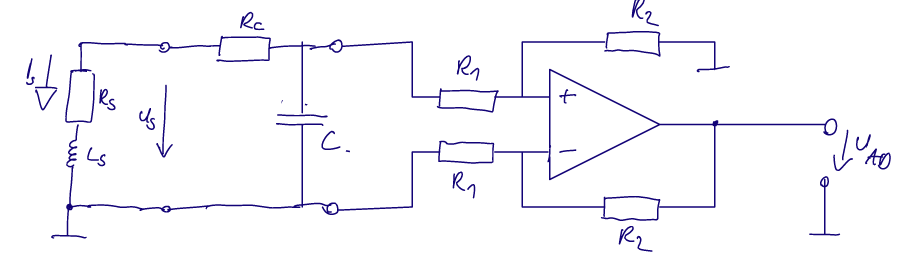
\includegraphics[width=1\linewidth]{Figures//tmp/42_schematic.png}
    \caption{Söntös árammérés mérőerősítővel}
    \label{fig:enter-label}
\end{figure}

1. lépésben határozzuk meg a szükséges erősítési paramétereket. Ehhez kiszámoljuk, hogy az áram mekkora feszültséget ejt az ellenálláson:

\begin{equation}
\begin{aligned}{}
    U_{s} &= R_s \cdot I_s = 10\; m\Omega{} \cdot 5\;A = \underline{50\; mV} \\
\end{aligned}
\end{equation}

Ebből pedig meg tudjuk határozni, hogy mekkora $G$ erősítésre lesz szükségünk:

\begin{equation}
\begin{aligned}{}
    G &= \frac{U_{AD}}{U_S} = \frac{5\;V}{50\;mV} = \underline{100} \\
\end{aligned}
\end{equation}

Innen pedig következnek a mérőerősítő kapcoslás ellenállás értékei. $R_1$-et válasszuk meg $10\;k\Omega$ értéknek.

\begin{equation}
\begin{aligned}{}
    G &= \frac{R_2}{R_1} \\
    R2 &= G \cdot R_1 = 100 \cdot 10\;k\Omega = \underline{1\;M\Omega} \\
\end{aligned}
\end{equation}

Ezek után már csak a sönt ellenállás parazita induktivitásának kompenzálása van hátra:


\begin{equation}
\begin{aligned}{}
    R_C \cdot C &= \frac{L_s}{R_s} \\
    C &= \frac{L_S}{R_S \cdot \R_C} = \frac{0,1\;\mu{H}}{10\;m\Omega \cdot 10\;\Omega} = \underline{1\;nF} \\
\end{aligned}
\end{equation}

\subsubsection{Galvanikusan leválasztott mérési elrendezések}

\begin{example}[\quad \large Analóg leválasztók 1.]

Egy váltakozó áramú motor áramát áramváltóval mérjük. A motor maximális felvett árama az 5Hz-100Hz frekvenciatartományban 10A. Az áramváltó áttétele 1:100, a szekunder oldalra vonatkoztatott mágnesezési induktivitása 1H. Legfeljebb mekkora sönt-ellenállással zárhatja le az áramváltót, ha a megengedett áramérzékelési hiba 1A?

\tcbline
\vspace{1mm}

\solution

\end{example}
\begin{example}[\quad \large Analóg leválasztók 2]

Rajzolja fel a kompenzációs elven működő Hall-elemes áramérzékelő és a hozzá kapcsolódó illesztő áramkör kapcsolását! A felhasznált Rs söntellenállás 1Ω, Np=1, Ns=1000, Ip=±100A, a jelfeldolgozó elektronika jeltartománya ±5V.

\tcbline
\vspace{1mm}

\solution

\end{example}
\begin{example}[\quad \large Analóg leválasztók 3]

Röviden ismertesse az egyszerű analóg optikai leválasztó(k) felépítését! Mit takar a CTR rövidítés? Mi a fő akadálya annak, hogy közvetlenül érzékelő áramkörben alkalmazzuk?

\tcbline
\vspace{1mm}

\solution

\end{example}
\begin{example}[\quad \large Analóg leválasztók 4]

Rajzolja fel a kompenzációs elven működő Hall-elemes áramérzékelő elvi kapcsolását! 
Méretezze a söntellenállást és az erősítőt! (Np=1, Ns=1000, Ip=±100A, a jelfeldolgozó elektronika jeltartománya ±5V és a söntellenállás maximális disszipációja 0,5W?


\tcbline
\vspace{1mm}

\solution

\end{example}
\begin{example}[\quad \large Analóg leválasztók 5.]

Tervezzen max. 10A-es amplitudójú áram érzékelésére alkalmas galvanikusan leválasztó érzékelőt analóg optikai csatoló felhasználásával. Az áramkör disszipációja max. 1W lehet, az optikai csatoló átviteli tényezője 0.01, max. LED árama 20mA. A kimeneti feszültségtartomány 0..5V legyen!


\tcbline
\vspace{1mm}

\solution

\end{example}
\begin{example}[\quad \large Analóg leválasztók 6]

Tervezzen max. 10A-es amplitudójú áram érzékelésére alkalmas galvanikusan leválasztó érzékelőt analóg optikai csatoló felhasználásával! A söntellenállás disszipációja max. 1W lehet, a söntellenállás induktivitása 0.1uH, az optikai csatoló átviteli tényezője 0.01, max. LED árama 20mA. A kimeneti feszültségtartomány 0..3V legyen!

\tcbline
\vspace{1mm}

\solution

\end{example}
\begin{example}[\quad \large Analóg leválasztók 6]

Tervezzen leválasztó erősítőt analóg optikai csatoló segítségével! Az erősítő 100mV-os bemenő tartományához a kimeneten 0..10V tartozzon.
Az optikai csatoló átviteli tényezője 0.01, maximális LED árama 20mA, a rendelkezésre álló tápfeszültség 15V-os.


\tcbline
\vspace{1mm}

\solution

\end{example}
\begin{example}[\quad \large Analóg leválasztók 7]

Egy 0-100Hz-es tartományban üzemelő frekvenciaváltó (inverter) kimeneti áramát kell érzékelnünk. Tervezzen és méretezzen olyan érzékelő áramkört, amely galvanikusan leválaszt, a maximum 10A-es kimeneti áram pillanatértéket feltételezve a szükséges mérési tartományban az árammal arányos jelet az A/D váltó 0-5V-os bemeneti tartományába konvertálja!

\tcbline
\vspace{1mm}

\solution

\end{example}


\subsection{Idő vagy frekvencia mérésre visszavezethető mérési eljárások}

\begin{example}[\quad \large Fordulatszám és pozíció érzékelés 1]

Egy adott alkalmazásban a fordulatszám-érzékeléssel szemben támasztott követelmények a következők:
\begin{itemize}
\item{} maximális fordulatszám: 1500 [fordulat/perc],
\item{} fordulatszám érzékelés felbontása 1:1000 ,
\item{} mintavételezési időköz: 1msec.
\end{itemize}
Megoldható-e a feladat inkrementális fordulatszámadóval? Miért? Javasoljon megoldást!

\tcbline
\vspace{1mm}

\solution

\end{example}
\begin{example}[\quad \large Fordulatszám és pozíció érzékelés 2]

Mire való a Gray kód? Mit jelent egy abszolút jeladónál a 2*12 bites felbontás?

\tcbline
\vspace{1mm}

\solution

\end{example}
\begin{example}[\quad \large Fordulatszám és pozíció érzékelés 3.]

Hogyan és milyen mértékben növelhető meg az inkrementális jeladóval érzékelt fordulatszám felbontása?

\tcbline
\vspace{1mm}

\solution

\end{example}
\begin{example}[\quad \large Fordulatszám és pozíció érzékelés 4.]

Egy sin/cos jeladó fordulatonként 1024 periódust ad le csatornánként. Mi lesz az érzékelhető legkisebb szögeltérés, ha az analóg jeleket 6 bites pontossággal dolgozzuk fel?

\tcbline
\vspace{1mm}

\solution

\end{example}
\begin{example}[\quad \large Fordulatszám és pozíció érzékelés 5]

Inkrementális jeladó jeleit feldolgozó áramkört tervezünk. Rajzolja fel az FPGA-ban megvalósítandó áramkör elvi rajzát! Felhasználható elemek: D tárolók, 4 bemenetű 3 kimenetű kombinációs hálózat, két irányú szinkron számláló. Mire használható a kombinációs (logikai) hálózat 3. kimenete? Milyen logikai függvénnyel állítjuk elő?

\tcbline
\vspace{1mm}

\solution

\end{example}
\begin{example}[\quad \large Fordulatszám és pozíció érzékelés 6.]

Rajzolja fel 1ms-ra az inkrementális fordulatszámadó A és B jeleinek időfüggvényét számszerűen is helyes, ha D=1000 és n=60/perc!

\tcbline
\vspace{1mm}

\solution

\end{example}
\begin{example}[\quad \large Fordulatszám és pozíció érzékelés 7]

Melyek az inkrementális fordulatszámadó jeleinek átadására szolgáló fizikai rétegek? Melyiknek mi az előnye?

\tcbline
\vspace{1mm}

\solution

\end{example}
\begin{example}[\quad \large Fordulatszám és pozíció érzékelés 8.]

Egy abszolút jeladót SSI-n keresztül kötünk a központi irányító elektronikába. Milyen funkciójú vezetékeket találunk a jeladó csatlakozójában? Hány pólusú csatlakozóra lesz szükség?

\tcbline
\vspace{1mm}

\solution

\end{example}

\vspace{-1.5mm}
\newpage
\section{Beágyazott irányító rendszerek}
\vspace{5cm}
\subsection{Beágyazott irányító rendszerek típusai}

\subsection{Mikrovezérlő alapú rendszerek}

\subsection{Gyakran használt mikrovezérlő perifériák}

\subsubsection{AD Átalakítók}

\subsubsection{Timer és Capture perifériák}
Digitális irányító rendszerek esteében alapvető fontosságú a rendszer műküdését vezérlő úrajel jelenléte. Jelen fejezetben arra nem térünk ki, hogy ez az úrajel honnan származik, de úgy tekintjük, hogy jelen van a rendszerben, ismert a frekvenciája és a pontossága, amely segítségével lehetségessé válik idő és frekvenciamérési feladatok megvalósítása. 

\subsection{Beágyazott kommunikációs interfészek}

\subsection{Digitális kommunikációs vonalak felépítése}

Digitális eszközök közötti adatcserére az iparban szabványoks kommunikációs protokollokat, kommuinkációs formákat haszánlunk. Ezek rendkívül sokrétűek, az olvasó is találkozhat velük a mindennapjaiban, legyen szó egy FM rádióadásról, a GSM hálózatról, vagy egy Ethernet kapcsolatról. Ezek a kommunkációs eljárások különböző, standard rétegeket implementálnak, melyek akár fel is cserélhetőek egymás között. (Pl. TCP/IP alapú kapcsolat megvalósítható WiFi-n és vezetlekes Ethernet hálózaton is) Ilyen modellszerű leírást ad meg az Open Systems Interconnection model (OSI model) is.

\paragraph{Layer 1: Fizikai réteg}

A fizikai réteg azt határozza meg, hogy milyen fizikai közegen keresztül áramlik az információ az eszközök között. A fizikai réteg specifikálja, hogy vezetékes, vagy vezeték nélküli kapcsolatról van-e szó, az átvitt jelek sázmát, az elvárt feszültésgszinteket és időzítéseket, a moduláció módját. A fizikai réteg dönti el, hogy az adat mely irányba áramolhat, simplex (egy irányú), half duplex (időosztáyban két irányú), vagy full duplex (folyamatosan két irányú) kommunikációról beszélünk-e.

\paragraph{Layer 2: Adatkapcsolati réteg}

\begin{example}[\quad \large Zavarérzékenység]

A tanult soros kommunikációk fizikai rétegei közül melyek hasonlóak zavarérzékenység, ill. logikai működés szempontjából?


\end{example}

\subsubsection{I2C}

Az $I^2C$ (Inter-Integrated Circuit) egy szinkon, csomagkapcsolt soros kommunikációs forma, melyet 1982-ben definiált a Philips Semiconductor (ma NXP). Igen elterjed, általában nyomtatott áramkörön belül, a különböző digitális eszközök között használt kommunikációs forma. Több, kompatibilis változata is létezik, iylen pl. az SMBus.

Leggyakrabban külsö ADC-k, EEPROM-ok és egyéb Flash memóriák, digitális érzékelők,  vagy egyszerű kijelzők vezérlésésre alkalmazzák.

Az I2C kommunikáció fizikai rétege 2 vezetékeből áll, melyre a perifériák open-collectoros kimenetekkel csatlakoznak, emiatt a busz vezetékeit fel kell húzni tápfeszültésgre. A tápfeszültségre felhúzú ellenállás méretét a kommunikációs sebesség, illetve a buszon található eszközök kapcitív terhelése határozza meg. Ez azt is jelenti, hogy ha a buszon bármely ezköz lehúzza bármely vezetéket annak feszültsége 0 lesz. Ez a két vezeték az SCL, azaz az órajelet közvetítő vezeték, illetve az SDA azaz az adatot közvetítő vezeték. Mivel az I2C buszon jelek nem diferenciális jelvátvitellel közlekednek, hanem egy vezetéken, ami az elektronika közös referencia feszültségéhez (GND) képest változtatja az értékét, single-ended kommunikációs vonalnak nevezzük. I2C buszon a logikai magas szint a magas feszültségnek felel meg, míg a logikai alacsony szint, a kis feszültségnek. A MASTER egység az üzenetek kezdetét un. START bittel jelzi, amely nem más mint az SDA vezeték alacsony állapotba állítása az SCL vezeték lehúzása nélkül nélkül. A STOP bit hasonló logika mentén, az órajel fix magas állapota melletti SDA magasba állítást jelenti az üzenet végén.

\begin{figure}[htb]
\begingroup
\tikzset{}
 \centerline{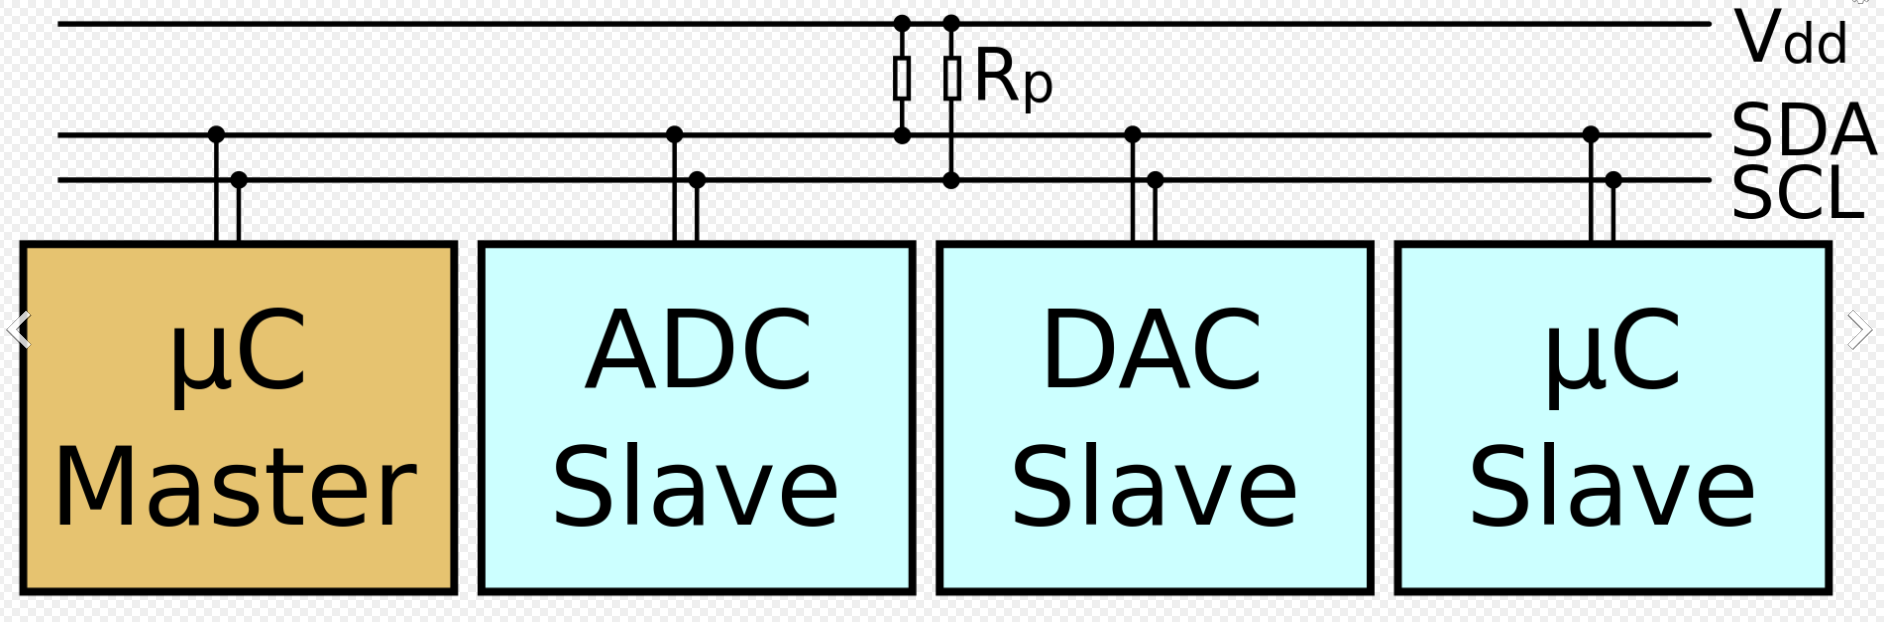
\includegraphics[width=0.6\columnwidth]{.//Figures/tmp/i2c_bus.png}}
 \endgroup
 \caption{I2C busz elrendezés}
 \label{fig:i2c_bus}
\end{figure}

A buszon két típusú eszköz található:
\begin{itemize}
    \item Master - ezen ezközök indítják a kommunikációt
    \item Slave - ezen eszközök reagálnak a kommunikációs kérdésekre
\end{itemize}

Egy buszon szerepelhet több master is, illetve a szerepeket akár dinamikusan is cserélhetik az eszközök, egyszerre azonban csak egyetlen eszköz adhat a buszon.

A buszon az eszközök alábbi üzemállapotokkal fordulhatnak elő:
\begin{itemize}
    \item master transmit
    \item master receive
    \item slave transmit
    \item slave receive
\end{itemize}

A buszon található különböző egységek megkülönböztetésére a cím szolgál. A master egység a START bit leadása után a MASTER elküldi a SLAVE egység 7 bites címét, majd ez után 1 bitben jelzi, ohgy írni (0), vagy olvasni (1) kíván az adott eszközbe/eszközből. Amennyiben a megcímzett SLAVE egység elérhető a buszon, így egy ACK bit kiadásával válaszol. A gyakorlatban ez az SDA vonal lehúzásást jeleni egy bit idejére.




\begin{example}[\quad \large I2C 1]

Ismertesse az I2C busz adatkapcsolati rétegét! Rajzoljon fel egy elrendezést 2 potenciális mester és 2 szolga résztvevővel! Vázolja fel a busz jeleit, ha a mester a 3 című eszközre egy 0 értékű és 255 értékű byte-ot ír és az eszköz képes a vételre!


\tcbline
\vspace{1mm}

\solution

\end{example}
\begin{example}[\quad \large I2C 2]

Ismertesse az I2C busz adatkapcsolati rétegét! Rajzoljon fel egy elrendezést 1 mester és 2 szolga résztvevővel! Vázolja fel a busz jeleit, ha a mester a 3 című eszközre egy 0 értékű byte-ot ír és az eszköz képes a vételre!


\tcbline
\vspace{1mm}

\solution

\end{example}
\begin{example}[\quad \large I2C 3]

Ismertesse az I2C busz adatkapcsolati rétegét! Rajzoljon fel egy elrendezést 1 mester és 2 szolga résztvevővel! Vázolja fel a busz jeleit, ha a mester a 127 című eszközre egy 0 értékű byte-ot ír és az eszköz képes a vételre!

\tcbline
\vspace{1mm}

\solution

\end{example}
\begin{example}[\quad \large I2C 4]

Ismertesse egy I2C buszos EEPROM egyetlen adatbájtja olvasásának fázisait.

\tcbline
\vspace{1mm}

\solution

\end{example}
\begin{example}[\quad \large I2C 5]

Rajzoljon fel egy elrendezést 1 mester és 2 szolga résztvevővel! Mi történik, ha a mester tévedésből két azonosra állított című eszközből olvas, ha az egyik eszközből olvasandó adat 0xaa, a másikból 0x55?

\tcbline
\vspace{1mm}

\solution

\end{example}


\subsubsection{SPI}

\begin{example}[\quad \large SPI 1]

Rajzoljon fel egy mestert és két szolgát tartalmazó rendszert! 

\tcbline
\vspace{1mm}

\solution

\end{example}
\begin{example}[\quad \large SPI 2]

Egy abszolút pozíció érzékelőt SSI interfészen illesztünk a folyamatirányító számítógéphez. Ismertesse a bekötéshez szükséges vezetékek szerepét! Melyik pillanatban érvényes pozíciót kapjak meg az irányító egység?

\tcbline
\vspace{1mm}

\solution

\end{example}
\begin{example}[\quad \large SPI 3]

Adja meg egy 4 bites adatok duplex átadásakor az SCLK, MOSI, MISO, CS (SL) jelek időfüggvényét!

\tcbline
\vspace{1mm}

\solution

\end{example}

\subsubsection{UART}

\begin{example}[\quad \large UART 1]

Rajzoljon fel egy 4 állomásos RS485-ös rendszert! 

\tcbline
\vspace{1mm}

\solution

\end{example}
\begin{example}[\quad \large UART 2]

Hasonlítsa össze az RS422 és az RS485 szabványokat!

\tcbline
\vspace{1mm}

\solution

\end{example}
\begin{example}[\quad \large UART 3]

Aszinkron soros kommunikáció alapszintű protokollja. Pl.: 7E2. 

\tcbline
\vspace{1mm}

\solution

\end{example}
\begin{example}[\quad \large UART 4]

Két processzor között aszinkron kommunikációt valósítunk meg. Megfelelnek-e a ±2,5\%-os pontosságú órajel-generátorok, ha a kommunikációs mód 8E1? Mikor lehet szükség egynél több stop bitre?

\tcbline
\vspace{1mm}

\solution

\end{example}
\begin{example}[\quad \large UART 5]

Rajzolja fel egy két részvevős RS485 rendszer vezetéke GND-hez képesti feszültségének időfüggvényét, amikor az egyik résztvevő 0x5A kódot küld 7O2 kommunikációs módban!

\tcbline
\vspace{1mm}

\solution

\end{example}
\begin{example}[\quad \large UART 6]

Rajzoljon fel egy 4 résztvevős RS485 szabvány szerinti kommunikációs rendszert! Mit érzékelnek a vevők, ha egyik részvevő sem ad?

\tcbline
\vspace{1mm}

\solution

\end{example}

\subsubsection{CAN}

\begin{example}[\quad \large CAN 1]

Mi a soros és a párhuzamos visszaverődés-mentesítés? Mikor melyiket célszerű alkalmazni?

\tcbline
\vspace{1mm}

\solution

\end{example}
\begin{example}[\quad \large CAN 2]

Egy CAN buszon két eszköz egyszerre kezd adni egy-egy standard ID-jű üzenetet. Az első eszköz üzenetének azonosítója 120, a másiké 64. Rajzolja fel az első eszköz TX és RX jelének első 12 bitjét!

\tcbline
\vspace{1mm}

\solution

\end{example}
\begin{example}[\quad \large CAN 3]

Egy CAN buszon két eszköz egyszerre kezd adni egy-egy standard ID-jű üzenetet. Az első eszköz üzenetének azonosítója 2047, a másiké 0. Rajzolja fel az első eszköz TX és RX jelének első 8 bitjét! Rajzoljon fel egy 4 résztvevős RS485 szabvány szerinti kommunikációs rendszert!

\tcbline
\vspace{1mm}

\solution

\end{example}
\begin{example}[\quad \large CAN 4]

CAN buszon az 1. állomás átviteli sebességét 500kBaudra állítottuk, a 2. állomás sebességét 1MBaud-ra. Mi lesz a 2. állomás TxD és RxD jele az első 10us-ban, ha az 1. állomás ID=3 azonosítójú üzenetet kezd el küldeni?

\tcbline
\vspace{1mm}

\solution

\end{example}
\begin{example}[\quad \large CAN 5]

Mit jelent a bit szintű arbitráció? A CAN üzenet melyik része az arbitrációs mező?

\tcbline
\vspace{1mm}

\solution

\end{example}
\begin{example}[\quad \large CAN 6]

Hány bites a DLC mező. Miért?

\tcbline
\vspace{1mm}

\solution

\end{example}
\begin{example}[\quad \large CAN 7]

Hány bites a standard ID? Mit jelent az, hogy a CAN üzenet-orientált?

\tcbline
\vspace{1mm}

\solution

\end{example}
\begin{example}[\quad \large CAN 8]

Ismertesse a CAN (A) üzenet felépítését! Hogyan változik meg a buszon mérhető jelsorozat, ha az egyik aktív ill. passzív vevő a CRC-t hibásnak érzékeli? 

\tcbline
\vspace{1mm}

\solution

\end{example}
\begin{example}[\quad \large CAN 9]

Mi az “error frame” és mikor adja egy résztvevő?

\tcbline
\vspace{1mm}

\solution

\end{example}
\begin{example}[\quad \large CAN 10]

Két processzor között CAN kommunikációt valósítunk meg. Megfelelnek-e a ±2,5\%-os pontosságú órajel-generátorok? 

\tcbline
\vspace{1mm}

\solution

\end{example}


\vspace{-1.5mm}
\newpage
\section{Bevezetés a teljesítményelektronikába}
\vspace{5cm}
\subsection{Teljesítményelektronikai félvezető elemek}
\subsubsection{Dióda}
\subsubsection{IGBT}
\subsubsection{FET}

\subsection{Lineáris üzemű tápegységek}


\subsection{Kapcsoló üzemű tápegységek}
\subsubsection{Buck-konverter}
\subsubsection{1 fázisú inverterek}
\subsubsection{3 fázisú inverterek}

\subsection{Kapcsoló üzemű táőegységek digitális irányítása}

\begin{example}[\quad \large DC/DC 1]

Egy DC motort 10kHz-es kapcsolási frekvenciájú hídkapcsolású DC-DC átalakítóról táplálunk. A DC feszültség 110V, a motor névleges feszültsége 100V, induktivitása 1mH, névleges fordulatszáma 1000ford/perc. Mekkora lesz az áramhullámosság álló motornál a tanult két modulációs módszernél?

\tcbline
\vspace{1mm}

\solution

\end{example}
\begin{example}[\quad \large DC/DC 2]

Egy hídkapcsolású DC-DC átalakítót eltolásos PWM-mel vezérlünk. Adja meg a „v” vezérlőjel és a kimeneti feszültség középértéke közötti kapcsolatot mindkét áramirány figyelembevételével, ha a „k” háromszög vivőjel 0V és 10V között változik, fsw = 10kHz, tdon=1us, tdoff=1,5us, td=3us, Uin=100V! 

\tcbline
\vspace{1mm}

\solution

\end{example}
\begin{example}[\quad \large DC/DC 3]

Egy hídkapcsolású DC-DC átalakítót eltolásos PWM-mel vezérlünk. Adja meg a „v” vezérlőjel és a kimeneti feszültség középértéke közötti kapcsolatot mindkét áramirány figyelembevételével, ha a „k” háromszög vivőjel 0V és 10V között változik, fsw = 10kHz, tdon=1us, tdoff=1,5us, td=3us, Uin=100V! 

\tcbline
\vspace{1mm}

\solution

\end{example}
\begin{example}[\quad \large DC/DC 4]

Egy DC motort 15kHz-es kapcsolási frekvenciájú hídkapcsolású DC-DC átalakítóról táplálunk. A DC feszültség 200V, a motor névleges feszültsége 100V, induktivitása 1mH, névleges fordulatszáma 1000ford/perc. Mekkora fordulatszámon lesz maximális a nyomatéklüktetés, ha ellenütemű vezérlést alkalmazunk? Mekkora lesz az áramhullámosság maximuma?

\tcbline
\vspace{1mm}

\solution

\end{example}
\begin{example}[\quad \large DC/DC 5]

Egy DC motort 5kHz-es kapcsolási frekvenciájú hídkapcsolású DC-DC átalakítóról táplálunk. A DC feszültség 120V, a motor névleges feszültsége 100V, induktivitása 1mH, névleges fordulatszáma 1000ford/perc. Mekkora fordulatszámon lesz maximális a nyomatéklüktetés, ha ellenütemű vezérlést alkalmazunk? Mekkora lesz az áramhullámosság maximuma?

\tcbline
\vspace{1mm}

\solution

\end{example}
\begin{example}[\quad \large DC/DC 6]

Mekkora lesz az egyfázisú hídkapcsolású inverter kimenőfeszültségének ötödik felharmónikusa, ha a kapcsoló elemek késleltetése ki és bekapcsolásnál 1-1usec, az egy ágban levő kapcsoló elemek vezérlése közötti holtidő 2usec (mindig a bekapcsolást késleltetjük), a kapcsolási frekvencia 10kHz, a bemeneti DC feszültség 100V és a terhelés soros R-L? 

\tcbline
\vspace{1mm}

\solution

\end{example}
\begin{example}[\quad \large DC/DC 7]

Egy egyfázisú hídkapcsolású invertert 300V-os egyenfeszültséggel táplálunk. Mekkora lesz ideális esetben a terhelésre jutó feszültség alapharmonikusának effektív értéke a szinuszos kivezérelhetõség határán? Hogyan változik meg a kimenőfeszültség alapharmonikusának effektív értéke, ha a kapcsoló elemek késleltetése ki és bekapcsolásnál 1-1usec, az egy ágban levõ kapcsoló elemek vezérlése közötti holtidõ 2usec, a kapcsolási frekvencia 10kHz és a kimeneti áram alapharmonikusa kb. azonos fázisú a fázisfeszültséggel?

\tcbline
\vspace{1mm}

\solution

\end{example}
\begin{example}[\quad \large DC/DC 8]

Egyfázisú szinuszos PWM vezérlésű DC-AC átalakító jellemzői:
fsw = 10kHz, tdon=1us, tdoff=1us, td=3us, UDC=100V.
Mekkora a harmadik harmonikus feszültség összetevő, ha a kitöltési tényező:
d=0.5*sin(wt) szerint változik?


\tcbline
\vspace{1mm}

\solution

\end{example}
\begin{example}[\quad \large DC/DC 9]

Egyfázisú szinuszos PWM vezérlésű DC-AC átalakító jellemzői:
fsw = 10kHz, tdon=1us, tdoff=1us, td=3us, UDC=100V.
Mekkora a harmadik harmonikus feszültség összetevő, ha a kitöltési tényező:
d=0.5*sin(wt) szerint változik?



\tcbline
\vspace{1mm}

\solution

\end{example}
\begin{example}[\quad \large DC/DC 10]

Egy egyfázisú hídkapcsolású inverter kapcsolási frekvenciája 10kHz, kimenőfeszültségének 5. felharmónikusa 5V, a kimenőáram 10kHz-es összetevője elhanyagolható, 20kHz-es összetevője 0.5A. Milyen vezérlési módszert használtunk? Mekkora lesz közelítőleg a kimenőfeszültség 5. felharmónikusa és a legjelentősebb nagyfrekvenciás összetevője, ha a kapcsolási frekvenciát 15kHz-re emeljük? Indoklás! 

\tcbline
\vspace{1mm}

\solution

\end{example}
\begin{example}[\quad \large DC/DC 11]

Egy háromfázisú hídkapcsolású inverter kapcsolási frekvenciája 10kHz, kimenőfeszültségének ötödik felharmónikusa 5V, a kimenőáram 10kHz-es összetevője 1A. Mekkora lesz közelítőleg a kimenőfeszültség ötödik felharmónikusa és a kimenőáram kapcsolási frekvenciás összetevője, ha a kapcsolási frekvenciát 15kHz-re emeljük? 

\tcbline
\vspace{1mm}

\solution

\end{example}
\begin{example}[\quad \large DC/DC 12]

Egy egyfázisú hídkapcsolású inverter kapcsolási frekvenciája 10kHz, kimenőfeszültségének harmadik felharmónikusa 5V, a kimenőáram 10kHz-es összetevője 1A. Milyen vezérlési módszert használtunk? Mekkora lesz közelítőleg a kimenőfeszültség harmadik felharmónikusa és a kimenőáram kapcsolási frekvenciás összetevője, ha a kapcsolási frekvenciát 15kHz-re emeljük? Indoklás!

\tcbline
\vspace{1mm}

\solution

\end{example}
\begin{example}[\quad \large DC/DC 13]

Hasonlítsa össze a ’flat-top’ moduláció és a 3. harmonikust tartalmazó modulációt a maximális kiadható szinuszos feszültség szempontjából! Hogyan hat a vezérlési holtidő az egyik ill. a másik esetben?

\tcbline
\vspace{1mm}

\solution

\end{example}
\begin{example}[\quad \large DC/DC 14]

Hasonlítsa össze a ’flat-top’ modulációt és a 3. harmonikust tartalmazó modulációt! Szempontok: kiadható szinuszos feszültség holtidő figyelembevételével, ill. anélkül,  kapcsolási veszteségek cos(fi)=1 feltételezésével, meghajtók táplálása. Időfüggvények.

\tcbline
\vspace{1mm}

\solution

\end{example}
\begin{example}[\quad \large DC/DC 15]

Hasonlítsa össze a Flat-top és a fázisonkénti szinuszos modulációt maximális kiadható szinuszos feszültség, kapcsolási veszteségek, alkalmazható meghajtó típus és felharmóniakusok szempontjából!

\tcbline
\vspace{1mm}

\solution

\end{example}
\begin{example}[\quad \large DC/DC 16]

Mekkora lesz a maximális kiadható szinuszos vonali feszültség csúcsértéke ’flat-top’, szimetrikus, fázisonkénti szinuszos és a 3. harmonikust tartalmazó moduláció alkalmazásakor, ha a DC feszültség értéke 600V?  Az utolsó módszernél mekkora lesz a harmadik harmonikus értéke?

\tcbline
\vspace{1mm}

\solution

\end{example}
\begin{example}[\quad \large DC/DC 17]

Mekkora DC feszültség szükséges a tanult modulációs módszereknél, ha a 400V-os háromfázisú motoron névleges feszültséget és szinuszos áramot akarunk biztosítani? Melyik modulációs módszernél a legalacsonyabb a szükséges DC feszültség, ha a holtidő hatását is figyelembe vesszük?

\tcbline
\vspace{1mm}

\solution

\end{example}
\begin{example}[\quad \large DC/DC 18]

Tüzelőanyag-cellával termelt energiát a 400V-os hálózatra szeretnénk visszatáplálni egy 3 fázisú inverter és egy 50Hz-es transzformátor felhasználásával. A tüzelőanyag-cella üzemi feszültsége 400V és 250V között változik. Mekkora áttételű transzformátoron keresztül csatlakozzunk a 10\%-os tűrésű hálózatra?

\tcbline
\vspace{1mm}

\solution

\end{example}
\begin{example}[\quad \large DC/DC 19]

Szimmetrikus (space vector) modulációt alkalmazó inverter alkalmazásban 400V vonali effektív értékű szinuszos feszültséget kell előállítanunk. Mekkora DC bemeneti feszültség szükséges? Mennyivel csökken a kiadott feszültség alapharmonikusa, ha változatlan vezérlés mellett a holtidőt is figyelembe vesszük (fsw = 10kHz, tdon=1us, tdoff=1us, td=3us, cos(fi)=1)? 

\tcbline
\vspace{1mm}

\solution

\end{example}
\begin{example}[\quad \large DC/DC 20]

Egy háromfázisú hídkapcsolású inverter bemeneti feszültsége 600V. Fázisonkénti szinuszos modulációt alkalmazunk, ahol az „a” fázis felső tranzisztorának kitöltési tényezője da=0,5+0,4*sin(2*π*50*t). A kapcsolási frekvencia 10kHz. Rajzolja fel a kapcsolást! Mekkora lesz a kimeneti feszültség alapharmonikus vonali feszültsége? A kimeneti vonali feszültséget spektrumanalizátorral vizsgálva 20V-os 250Hz-es összetevőt mérünk. Mi lehet ennek az oka?

\tcbline
\vspace{1mm}

\solution

\end{example}

\vspace{-1.5mm}
\newpage

%\begin{thebibliography}{}
	\vspace{4cm}
		\bibitem{RPI} Academic and Research Computing. \textit{Text Formatting with \LaTeX\ A Tutorial}. NY, April 2007.\\
				\url{http://www.rpi.edu/dept/arc/docs/latex/latex-intro.pdf}
		\bibitem{is.skills} Leslie Lamport. \textit{\LaTeX\ for Beginners}.  fifth edition, Document Reference: 3722-2014, March 2014.\\
				\url{http://www.docs.is.ed.ac.uk/skills/documents/3722/3722-2014.pdf}
		\bibitem{Tobias Oetiker} Tobias Oetiker, Hubert Partl, Irene Hyna, and Elisabeth Schlegl. \textit{The Not So Short Introduction to \LaTeX\ }. Version 6.3, March 1994.\\
				\url{https://tobi.oetiker.ch/lshort/lshort.pdf}
		\bibitem{Helmut Kopka} Helmut Kopka and Patrick W. Daly. \textit{A Guide to \LaTeX\ and Electronic Publishing}. Addison-Wesley, fourth edition, May 2003.\\
				\url{https://www2.mps.mpg.de/homes/daly/GTL/gtl_20030512.pdf}
		\bibitem{Philip Hirschhorn} Philip Hirschhorn. \textit{Using the exam document class}. Wellesley College, second edition, MA, November 2017.\\
				\url{http://www-math.mit.edu/~psh/exam/examdoc.pdf}
		\bibitem{web1} \textit{When should I use \cs{input} vs \cs{include}}.\\
				\url{https://tex.stackexchange.com/questions/246/when-should-i-use-input-vs-include}		
		\bibitem{Overleaf} Overleaf. \textit{Inserting Images}.\\
				\url{https://www.overleaf.com/learn/latex/Inserting_Images}
		\bibitem{Rice} Rice University. \textit{\LaTeX\ Mathematical Symbols}.\\
			\url{https://www.caam.rice.edu/~heinken/latex/symbols.pdf}
		\bibitem{Overleaf1} Overleaf. \textit{Integrals, sum and limits}.\\
			\url{https://www.overleaf.com/learn/latex/Integrals,_sums_and_limits}
		\bibitem{BU} Boston University. \textit{\LaTeX\ Command Summary}. December 1994.\\
			\url{https://www.bu.edu/math/files/2013/08/LongTeX1.pdf}
		\bibitem{Overleaf2} Overleaf. \textit{Subscripts and superscripts}.\\
			\url{https://www.overleaf.com/learn/latex/Subscripts_and_superscripts}
		\bibitem{Disquis} Disquis. \textit{\LaTeX\ Color}. Addison-Wesley, second edition, Reading, MA, 1994.\\
				\url{http://latexcolor.com/}
		\bibitem{David Woods} David Woods.\textit{Useful \LaTeX\ Commands}.\\
				\url{https://www.scss.tcd.ie/~dwoods/1617/CS1LL2/HT/wk1/commands.pdf}
		\bibitem{Overleaf3} Overleaf. \textit{Spacing in Math Mode}.\\
				\url{https://www.overleaf.com/learn/latex/Spacing_in_math_mode}
		\bibitem{Overleaf4} Overleaf. \textit{Fractions and Binomials}.\\
				\url{https://www.overleaf.com/learn/latex/Fractions_and_Binomials}
		\bibitem{Overleaf5} Overleaf. \textit{Environments}.\\
				\url{https://www.overleaf.com/learn/latex/Environments}
		\bibitem{Overleaf6} Overleaf. \textit{Margin Notes}.\\
				\url{https://www.overleaf.com/learn/latex/Margin_notes}
		\bibitem{Math} Art of Problem Solving. \textit{LaTeX:Commands}\\
				\url{https://artofproblemsolving.com/wiki/index.php/LaTeX:Commands}
		\bibitem{LaTeX} Latex-Project.\\
				\url{https://www.latex-project.org/about/}
		\bibitem{texstackexchange} Tex Stack Exchange. customizing part style with Tikz.\\
				\url{https://tex.stackexchange.com/questions/159551/customizing-part-style-with-tikz}
		\bibitem{texstackexchange2}	Tex Stack Exchange. How to change chapter/section style in tufte-book?.\\
				\url{https://tex.stackexchange.com/questions/83057/how-to-change-chapter-section-style-in-tufte-book?noredirect=1&lq=1}
	\end{thebibliography}
\addtocounter{section}{14}
\addcontentsline{toc}{section}{\protect\numberline{\thesection}~~~ References}


\end{document}